
\frame{
  \frametitle{``No-lose'' theorem(s)}
  \footnotesize

      La non-violazione dell'unitariet\`a \`e stata spesso sfruttata come guida per la ricerca di nuova fisica
      \begin{tabular}{c}
        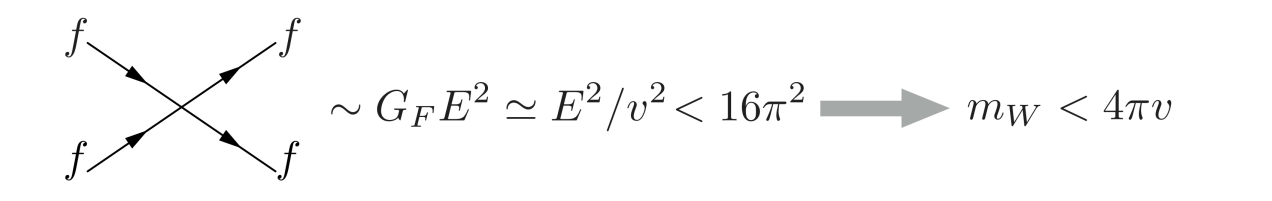
\includegraphics[width=0.6\linewidth]{figs/FermiNL.png}\\
        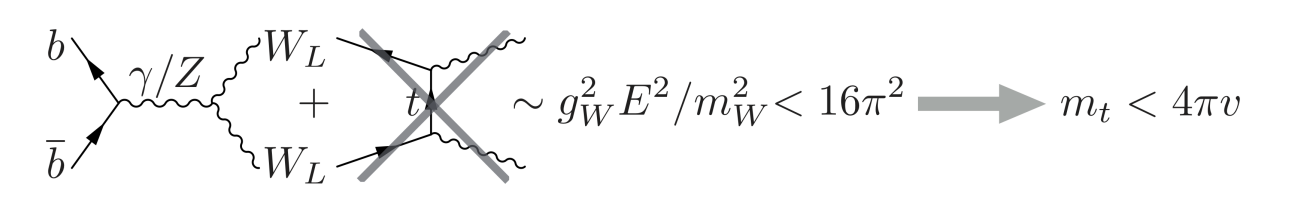
\includegraphics[width=0.6\linewidth]{figs/bbNL.png}\\
        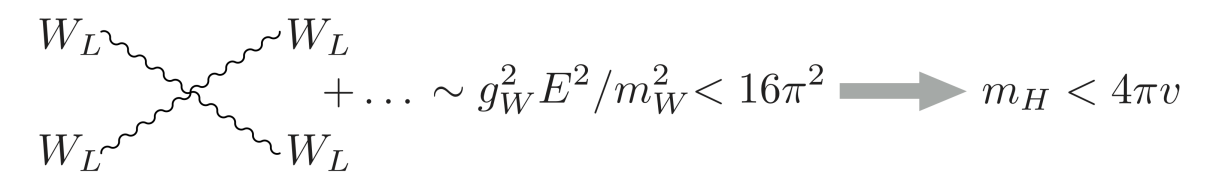
\includegraphics[width=0.6\linewidth]{figs/WWNL.png}\\
        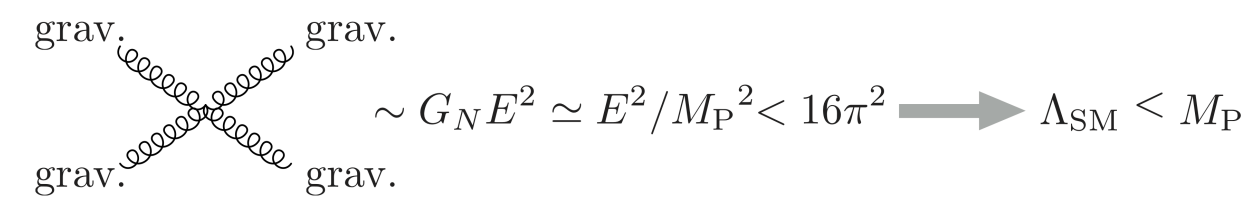
\includegraphics[width=0.6\linewidth]{figs/GravNL.png}
      \end{tabular}
      
  Con la scoperta del bosone di Higgs abbiamo una teoria (Modello Standard) valida, in teoria, fino alla scala di Planck.
}

\frame{
  \frametitle{Questioni aperte nel Modello Standard}
  \begin{itemize}
  \item Numero di parametri molto alto
    \begin{itemize}
      \item 12  masse fermioniche  (considerando i neutrini)
      \item 3   costanti di gauge
      \item 6+2 parametri di mixing (tre angoli e una fase (CP) per quark e neutrini)
      \item 1   fase per CP-forte
      \item 2   parametri per il settore di Higgs ($m_H$ e $\lambda$)
    \end{itemize}
  \item Le masse sono distribuite su un intervallo molto ampio (pi\`u o meno clusterizzate in famiglie)
  \item Il bosone di Higgs \`e l'unico scalare
  \item Non include la gravit\`a
  \end{itemize}
}

\frame{
  \frametitle{Divergenza nel termine di autoaccoppiamento del bosone di Higgs}
  \footnotesize
  Un problema legato in particolare al settore di Higgs \`e quello della gerachia. In particolare il termine di auto-interazione del bosone di Higgs diverge con la scala di Planck.
\vskip 0.1cm
  Bosoni e fermioni hanno masse vincolate dalla simmetria di gauge (devono andare a zero nel limite in cui la simmetria non \`e rotta). Il bosone di Higgs no.
\vskip 0.1cm
  Soluzione introduco una simmetria che vincoli a zero la correzione alla massa del bosone di Higgs.
  
      \begin{tabular}{c}
        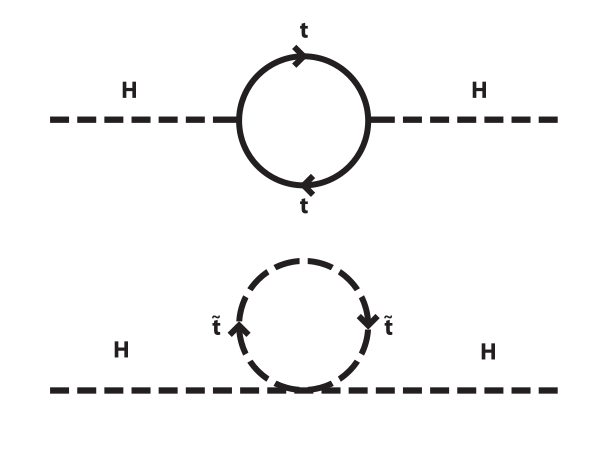
\includegraphics[width=0.5\linewidth]{figs/SusyCanc.png}
      \end{tabular}  
}


\frame{
  \frametitle{Supersimmetria}
  \footnotesize
      Per ogni particella del Modello Standard esiste una particella con statistica opposta (per ogni fermione esiste un bosone e viceversa)
      \begin{itemize}
      \item La simmetria deve essere ``rotta'' (spontaneamente come nel caso della simmetria SU(2)))
      \end{itemize}
  \begin{minipage}{0.45\linewidth}{
      \begin{itemize}
      \item Il nuovo ``cut-off'' \`e dato dalla scala di energia a cui si manifestano le nuove particelle.
      \item Se $\delta m_H \le m_H$ la cancellazione della divergenza nella massa dell'Higgs \`e ``naturale'', questo avviene se la scala a cui si manifestano le nuove particelle \`e dell'ordine del TeV.
      \end{itemize}
      
      }\end{minipage}\begin{minipage}{0.55\linewidth}{
  \begin{center}
    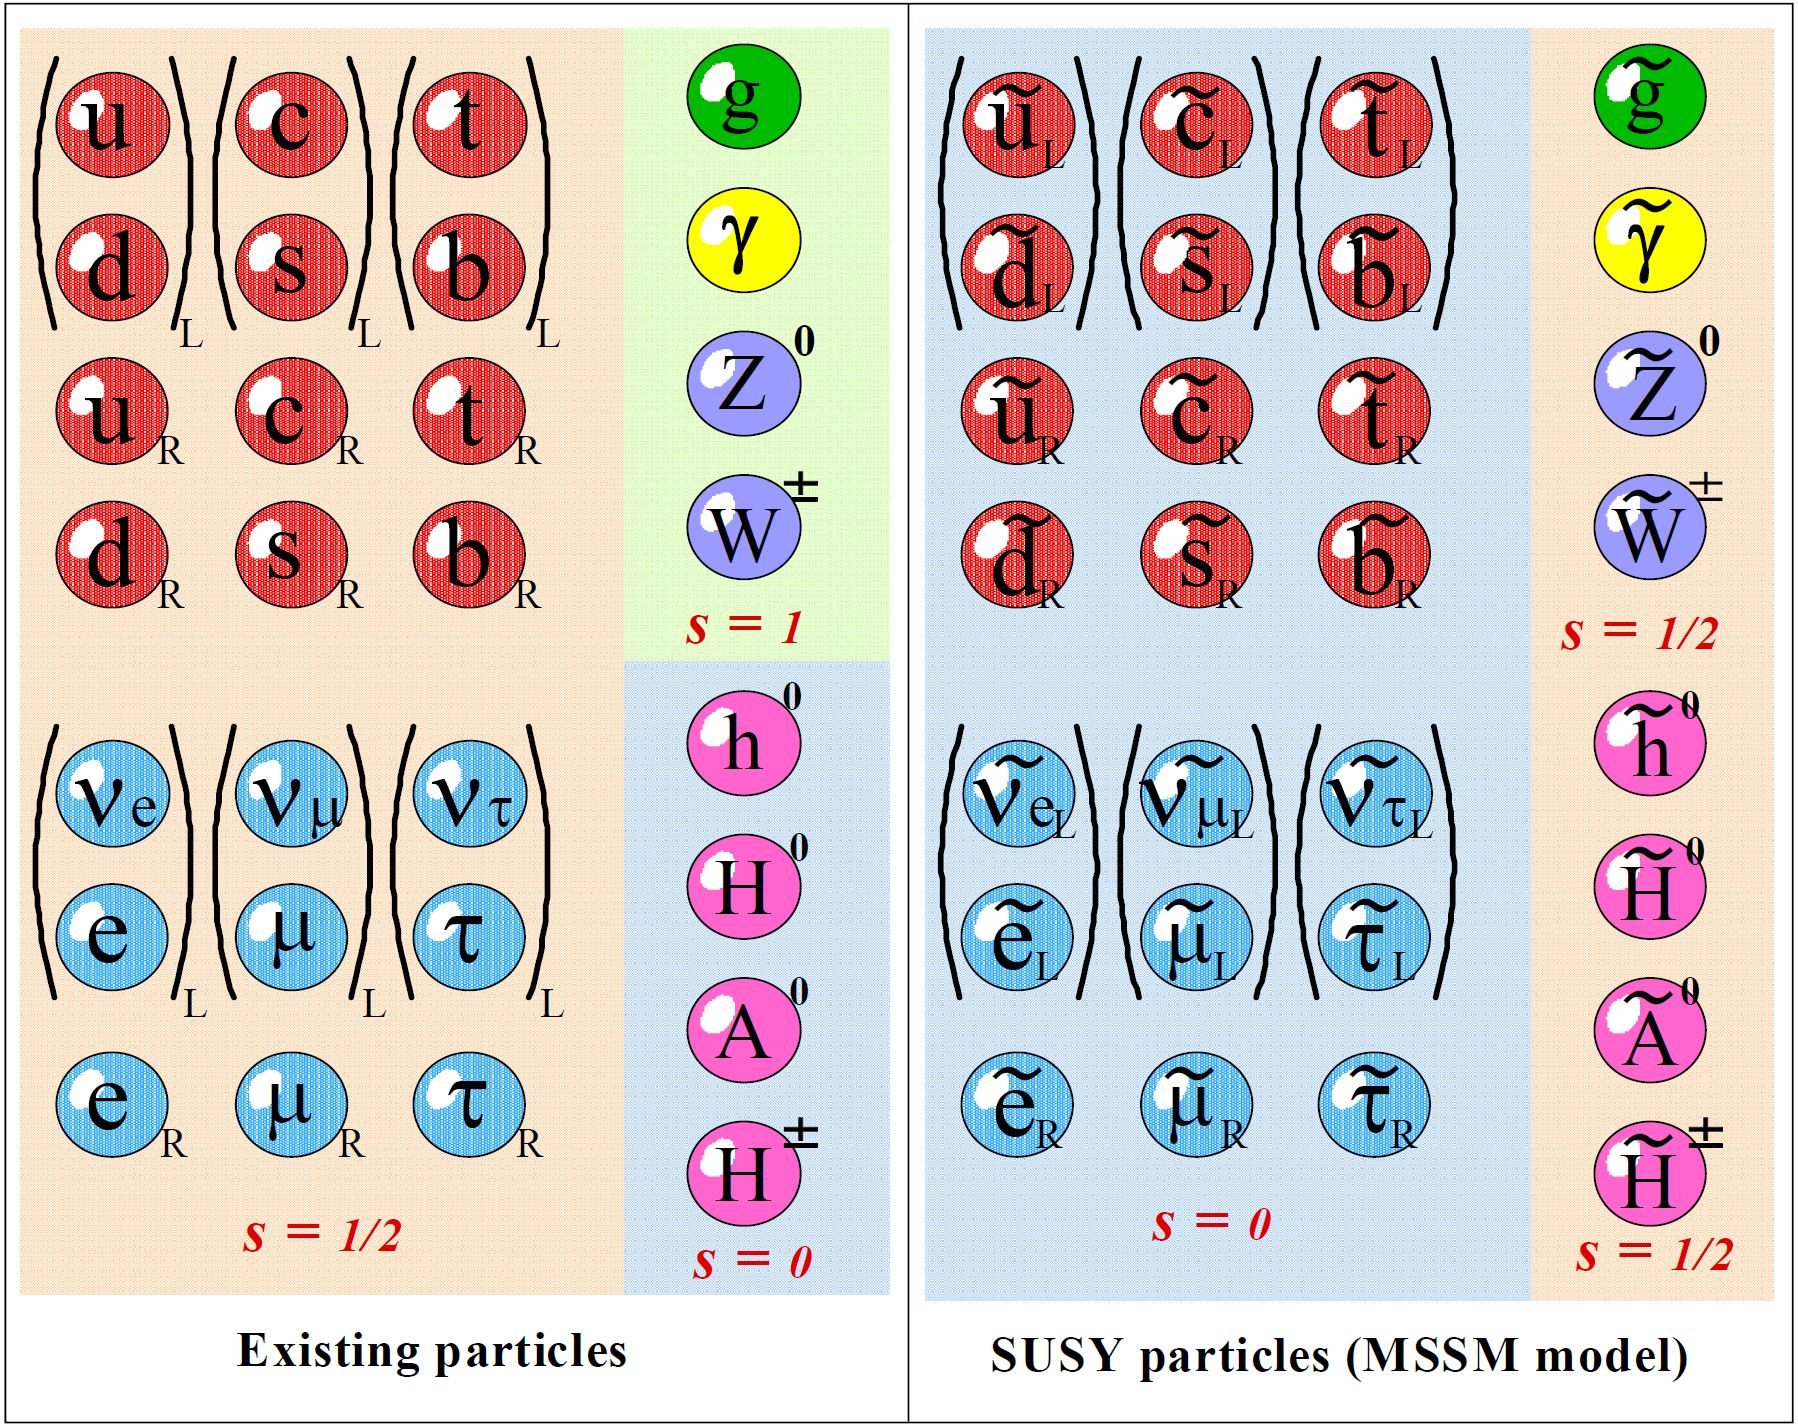
\includegraphics[width=0.9\linewidth]{figs/MSSM.jpg}
  \end{center}
  }\end{minipage}
}

\frame{
  \frametitle{Supersimmetria}
  \footnotesize
  Caratteristiche interessanti della Supersimmetria:
 \begin{itemize}
 \item La teoria delle stringhe \`e una teoria supersimmetria
 \end{itemize}
  
    \begin{minipage}{0.40\linewidth}{
        \begin{flushleft}
 \begin{itemize}
  \item Assumendo l'esistenza di  supersimmetria alla scale del TeV si ha una perfetta convergenza
   delle costanti di accoppiamento
 \end{itemize}
        \end{flushleft}
  }\end{minipage}\hfill\begin{minipage}{0.60\linewidth}{
  \begin{center}
    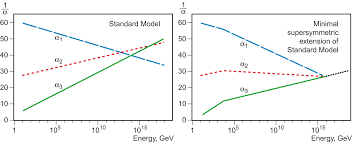
\includegraphics[width=0.8\linewidth]{figs/couplUni.png}
  \end{center}
    }\end{minipage}
    
 \begin{itemize}
  \item Unica simmetria compatibile con il gruppo di Lorentz non ancora verificata
    sperimentalmente.
 % \item Sono previsti 5 bosoni di Higgs: 3 neutri (h, H scalari e A pseudoscalare)
 %   e 2 carichi $H^{\pm}$
  \item Le particelle supersimmetriche decadono in particelle del Modello Standard e supersimmetriche. Nei modelli
    che conservano la R-parit\`a
    \vskip -0.5cm
    \begin{align*}
       R  = (-1)^{2B+L-2S}
    \end{align*}
    esiste una particella supersimmetrica stabile neutra (neutralino: mix dei super-patner
    di Z, fotone e Higgs neutri): candidato ideale per DM !
  \end{itemize}
  Caratteristiche meno interessanti della Supersimmetria:
  \begin{itemize}
    \item Al momento non c'\`e evidenza sperimentale
 \end{itemize}
}

\frame{
  \frametitle{Ricerche di Supersimmetria}
  \begin{itemize}
  \item Molte diverse segnature (anche in funzione dello specifico modello)
  \begin{tabular}{cc}
    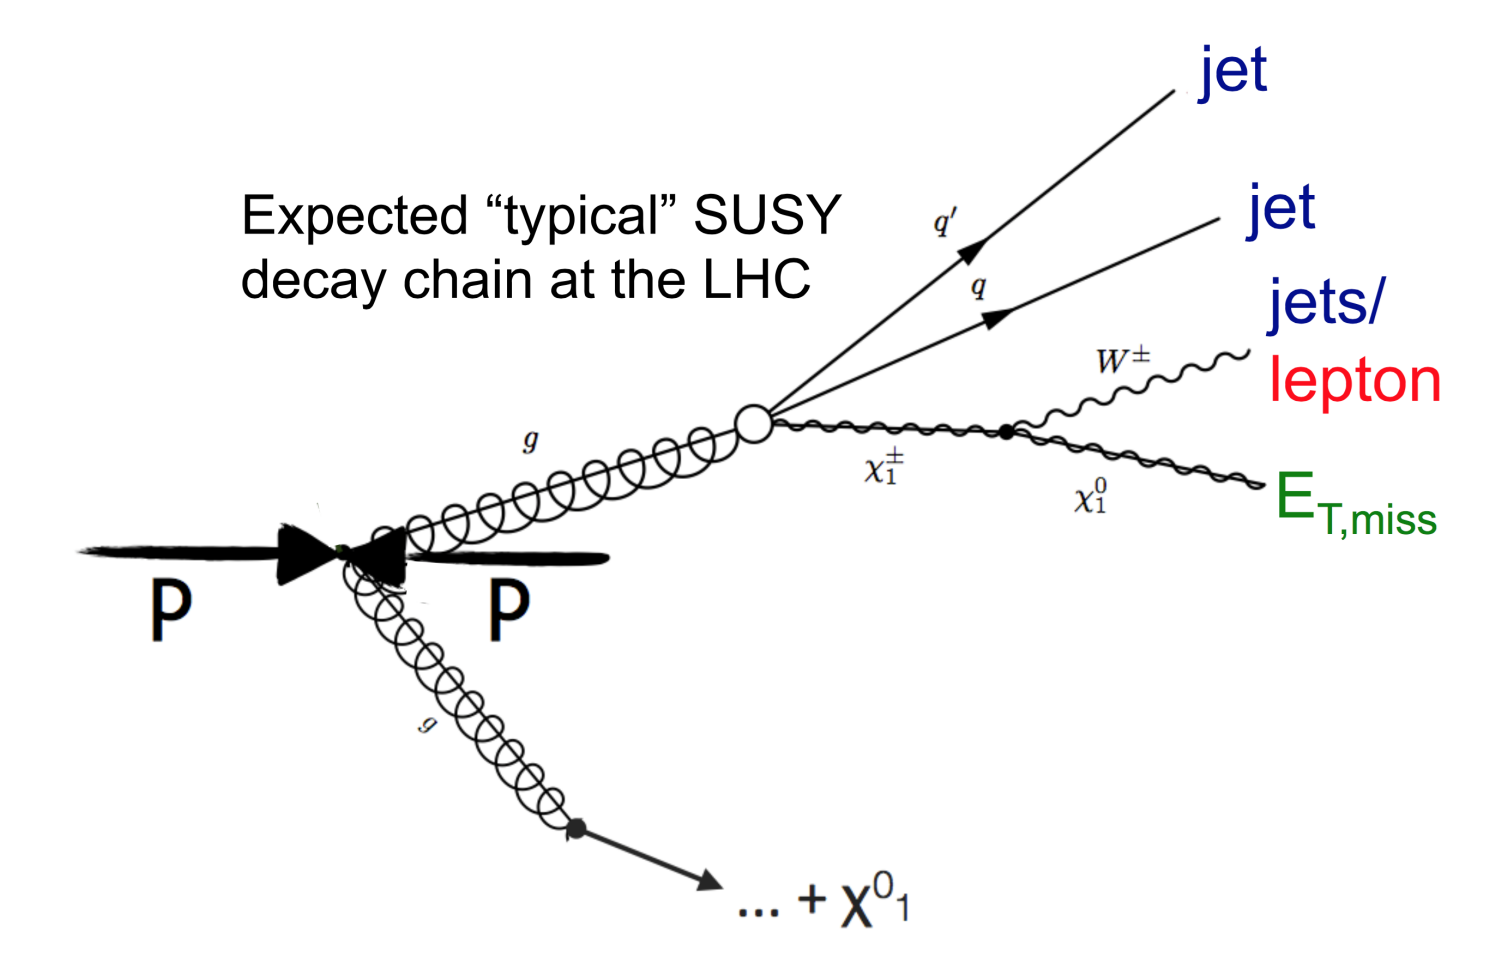
\includegraphics[width=0.4\linewidth]{figs/SUSYSign.png} &
    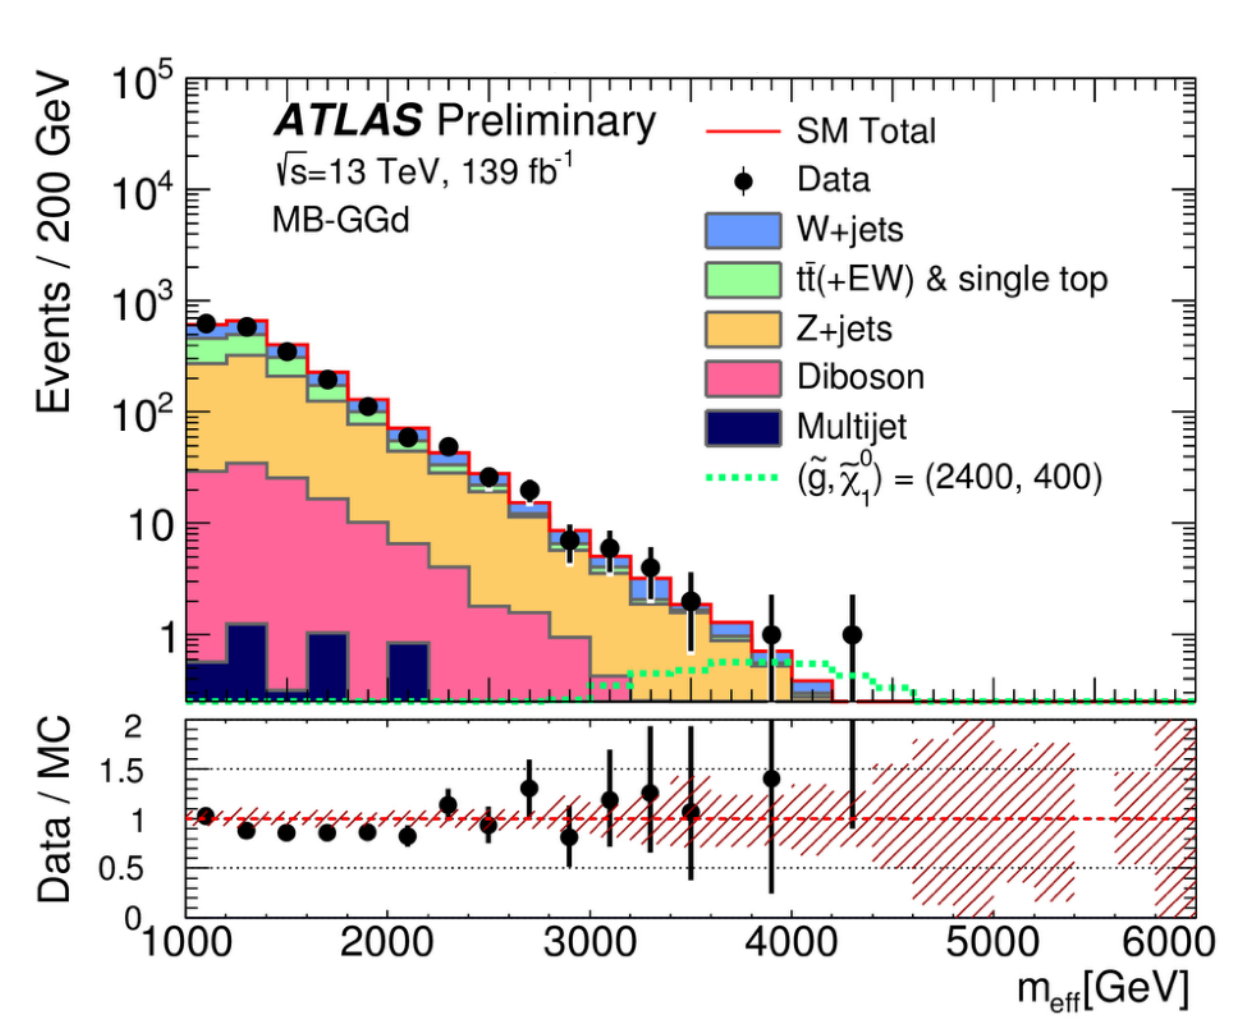
\includegraphics[width=0.4\linewidth]{figs/SUSYS.png}
  \end{tabular}
  \item Nello stato finale \`e sempre presente energia mancante (+ jets/leptoni)
  \item Analisi in funzione di energia mancante o massa efficace ($m_{eff}=\sum_i |p^T_i| + E^T_{miss}$)
  \end{itemize}
}

\frame{
  \frametitle{Ricerche di Supersimmetria}

  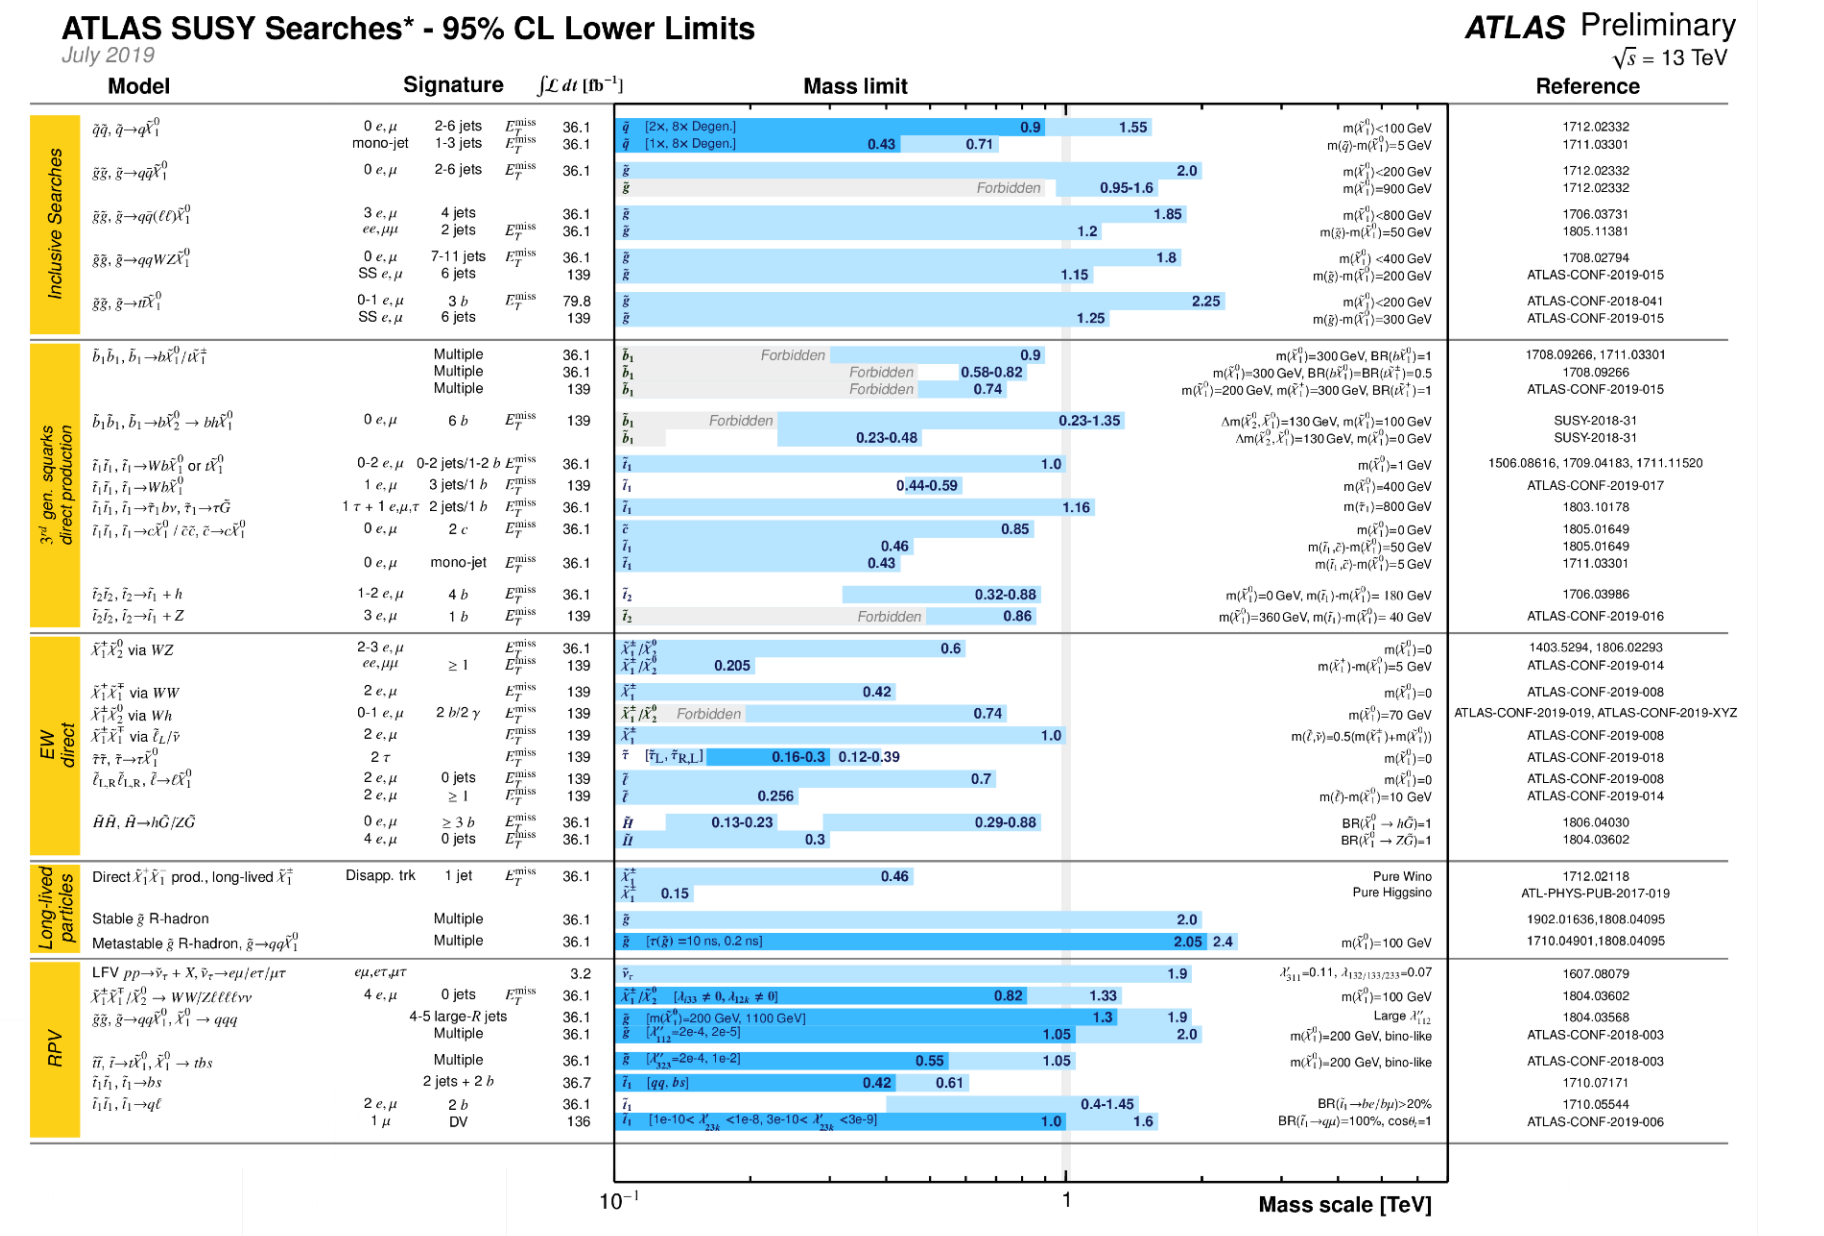
\includegraphics[width=0.6\linewidth]{figs/SuSum.png}
  
  Molti limiti sono gi\`a a livello del TeV o oltre.
}

\frame{
  \frametitle{Ricerche di Supersimmetria}
  \footnotesize
  
  Tuttavia lo spazio dei parametri, nella maggior parte delle ricerche, \`e lontano
  dall'essere coperto.

  \vskip 0.1cm
  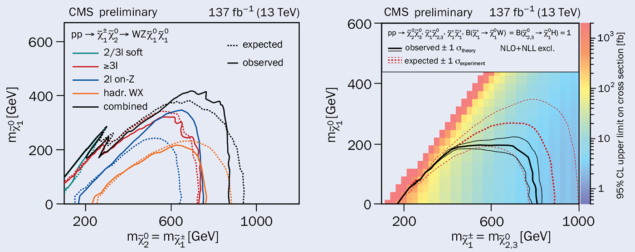
\includegraphics[width=0.8\linewidth]{figs/CMSSUSY.jpeg}

}



%\frame{
%  \frametitle{Misure di precisione (inaspettate)}
%  La recente misura di precisione della massa del W ha evidenziato una discrepanza (che andr\`a verificata)
%  con i risultati ottenuti dagli altri esperimenti e con il fit globale ai dati electroweak
%    \includegraphics[width=0.6\linewidth]{boson1.jpg}
%}

%\frame{
%  \frametitle{Misure necessarie per le misure di precisione}
%  Per fare misure di precisione servono altre misure (che magari non contengono elementi di nuova fisica)
%  che costituiscono una sorgente sistematica rilevante per le prime.
%  \vskip 0.5cm
%  Ad es. le pdf:\\
%    \includegraphics[width=0.6\linewidth]{ggF_pdf.png}
%}

\frame{
  \frametitle{Misure di precisione vs ricerca diretta}
  \footnotesize
  \begin{itemize}
  \item Le misure di precisione possono essere utili per evidenziare stati di altissima massa (non raggiungibile direttamente), gli effetti nei loop sono
    spesso proporzionali alla massa.
  \item Spesso tuttavia una misura di precisione indica solo un ``scostamento'' che deve poi essere interpretato in qualche modello teorico
    \begin{itemize}
      \footnotesize
    \item  EFT: Effective Field Theory: classifico i contributi ad un processo in termini di extra operatori generici. Determino i pi\`u significativi
      sulla base dei dati. Identifico una teoria coerente con quei contributi
    \end{itemize}
  \item Analisi completamente model independent: sulla base di tutti i dati misurati (in tutte le distribuzioni) determino se esistono scostamenti dal MS
    \begin{itemize}
      \footnotesize
    \item Multidimensionale: Machine Learning
    \item Sforzo da parte sperimentale per rendere disponibili tutti i dati in un formato comune.
    \end{itemize}
  \end{itemize}
}

\frame{
  \frametitle{Misure di precisione: prospettive sperimentali}
  \footnotesize
  \begin{itemize}
  \item HL LHC rappresenta un'opportunit\`a unica per misure di precisione (altissima luminosit\`a) nonostante
        sia una macchina adronica
      \item Tuttavia il miglioramente non \`e mai solo statistico. Anche le incertezza sistematiche
        diminuiscono perch\'e legate a misure ancillari che vengono, anch'esse migliorate
        (pdf, calibrazioni, etc..)

        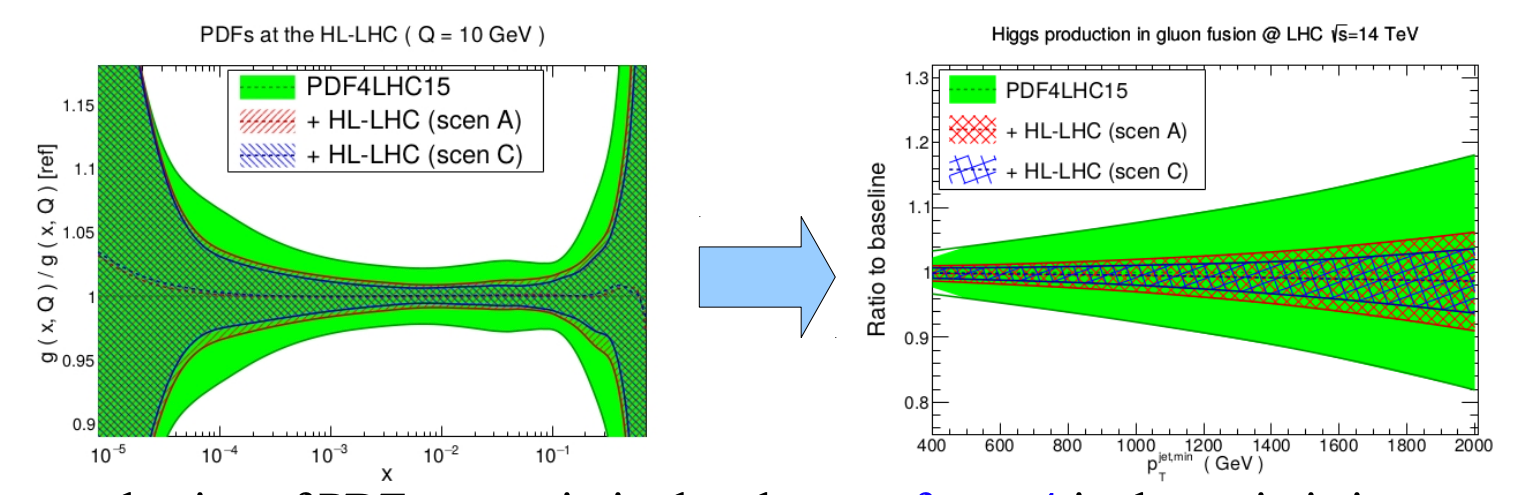
\includegraphics[width=0.6\linewidth]{figs/HLLHC_pdf.png}
        
    \item Inoltre nuove tecniche e/o nuove idee possono aprire la possibilit\`a di balzi di sensitivit\`a enormi.
  \end{itemize}
}

\frame{
  \frametitle{Misure di precisione dell'Higgs}
  \footnotesize
  \begin{itemize}
  \item Unica particella scalare: essenziale misurare con precisione tutti i parametri.
  \item Nei modelli supersimmetrici sono previsti 5 bosoni di Higgs: 3 neutri (h, H scalari e A pseudoscalare)
        e 2 carichi $H^{\pm}$
  \item Misure di precisione dei decadimenti del bosone di Higgs possono evidenziare
        un comportamento diverso da quello previsto dal ``puro'' Modello Standard
   \end{itemize}
  \begin{center}
    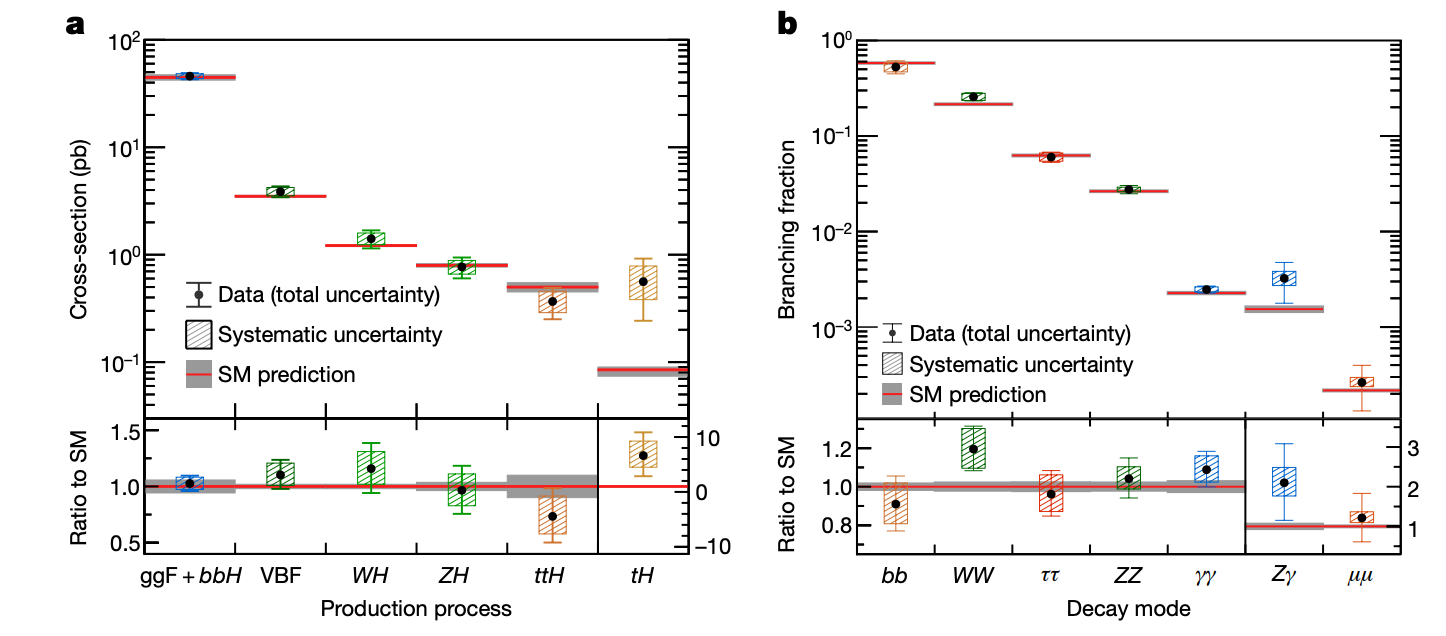
\includegraphics[width=0.7\linewidth]{figs/HiggsX.png}
  \end{center}
}

\frame{
  \frametitle{Misure di precisione dell'Higgs: HL LHC}
  \footnotesize
  \begin{minipage}{0.45\linewidth}{
      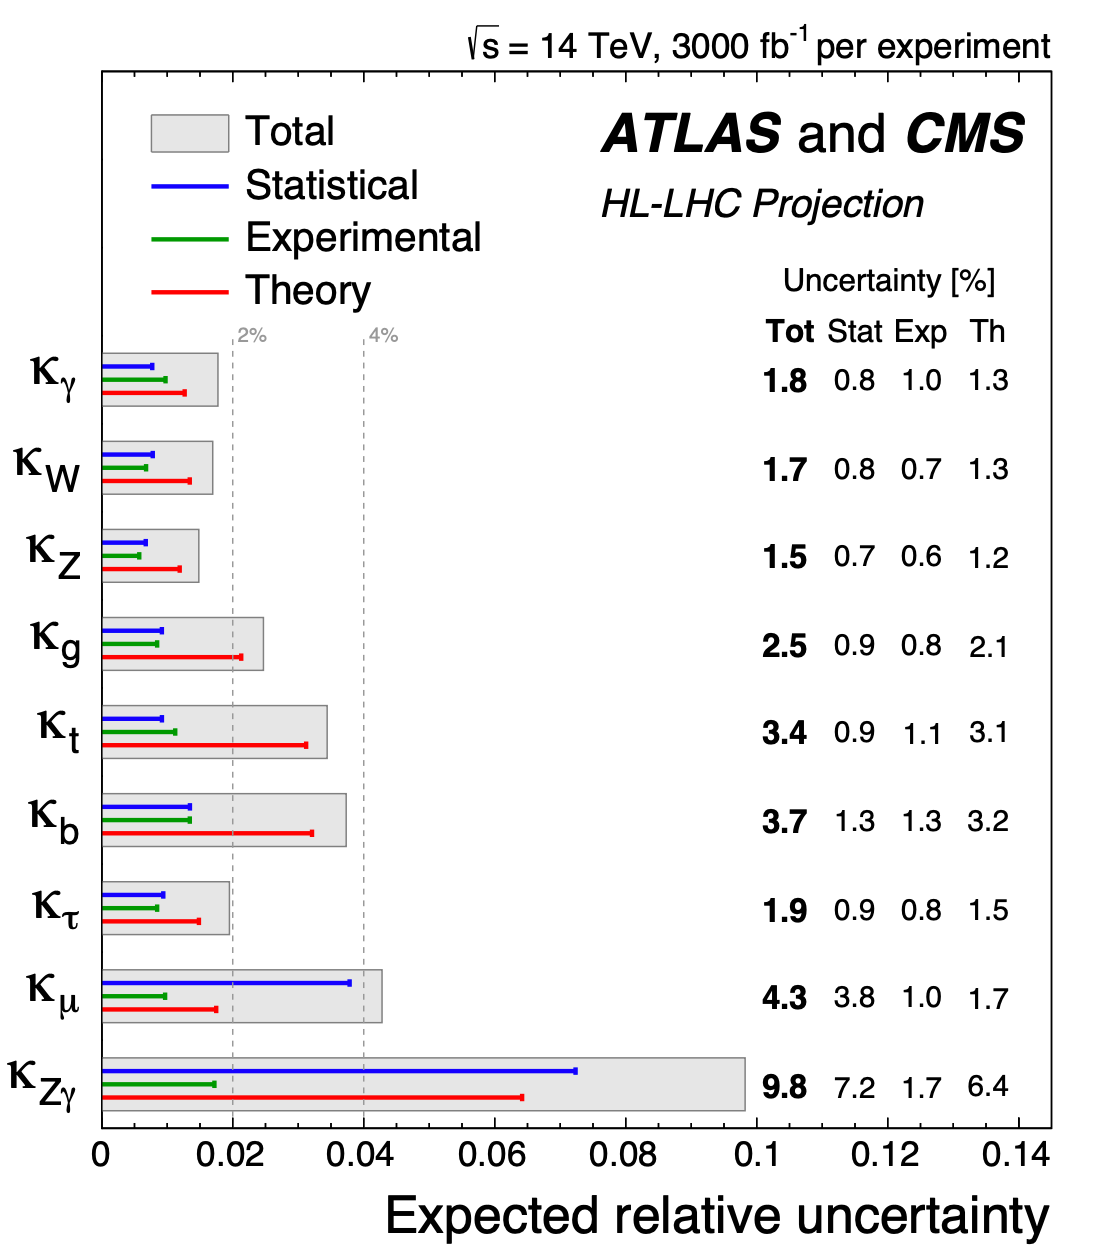
\includegraphics[width=0.9\linewidth]{figs/HiggsCoup.png}
  }\end{minipage}\hfill\begin{minipage}{0.55\linewidth}{
      \begin{itemize}
      \item Tutti i coupling al \%
      \item Misura $H\rightarrow c\bar c$ (progressi rilevanti nell'ultimo anno)
      \item Misura di $\Gamma_H$ al 20\% (misura preliminare tramite interfenza)
      \end{itemize}
      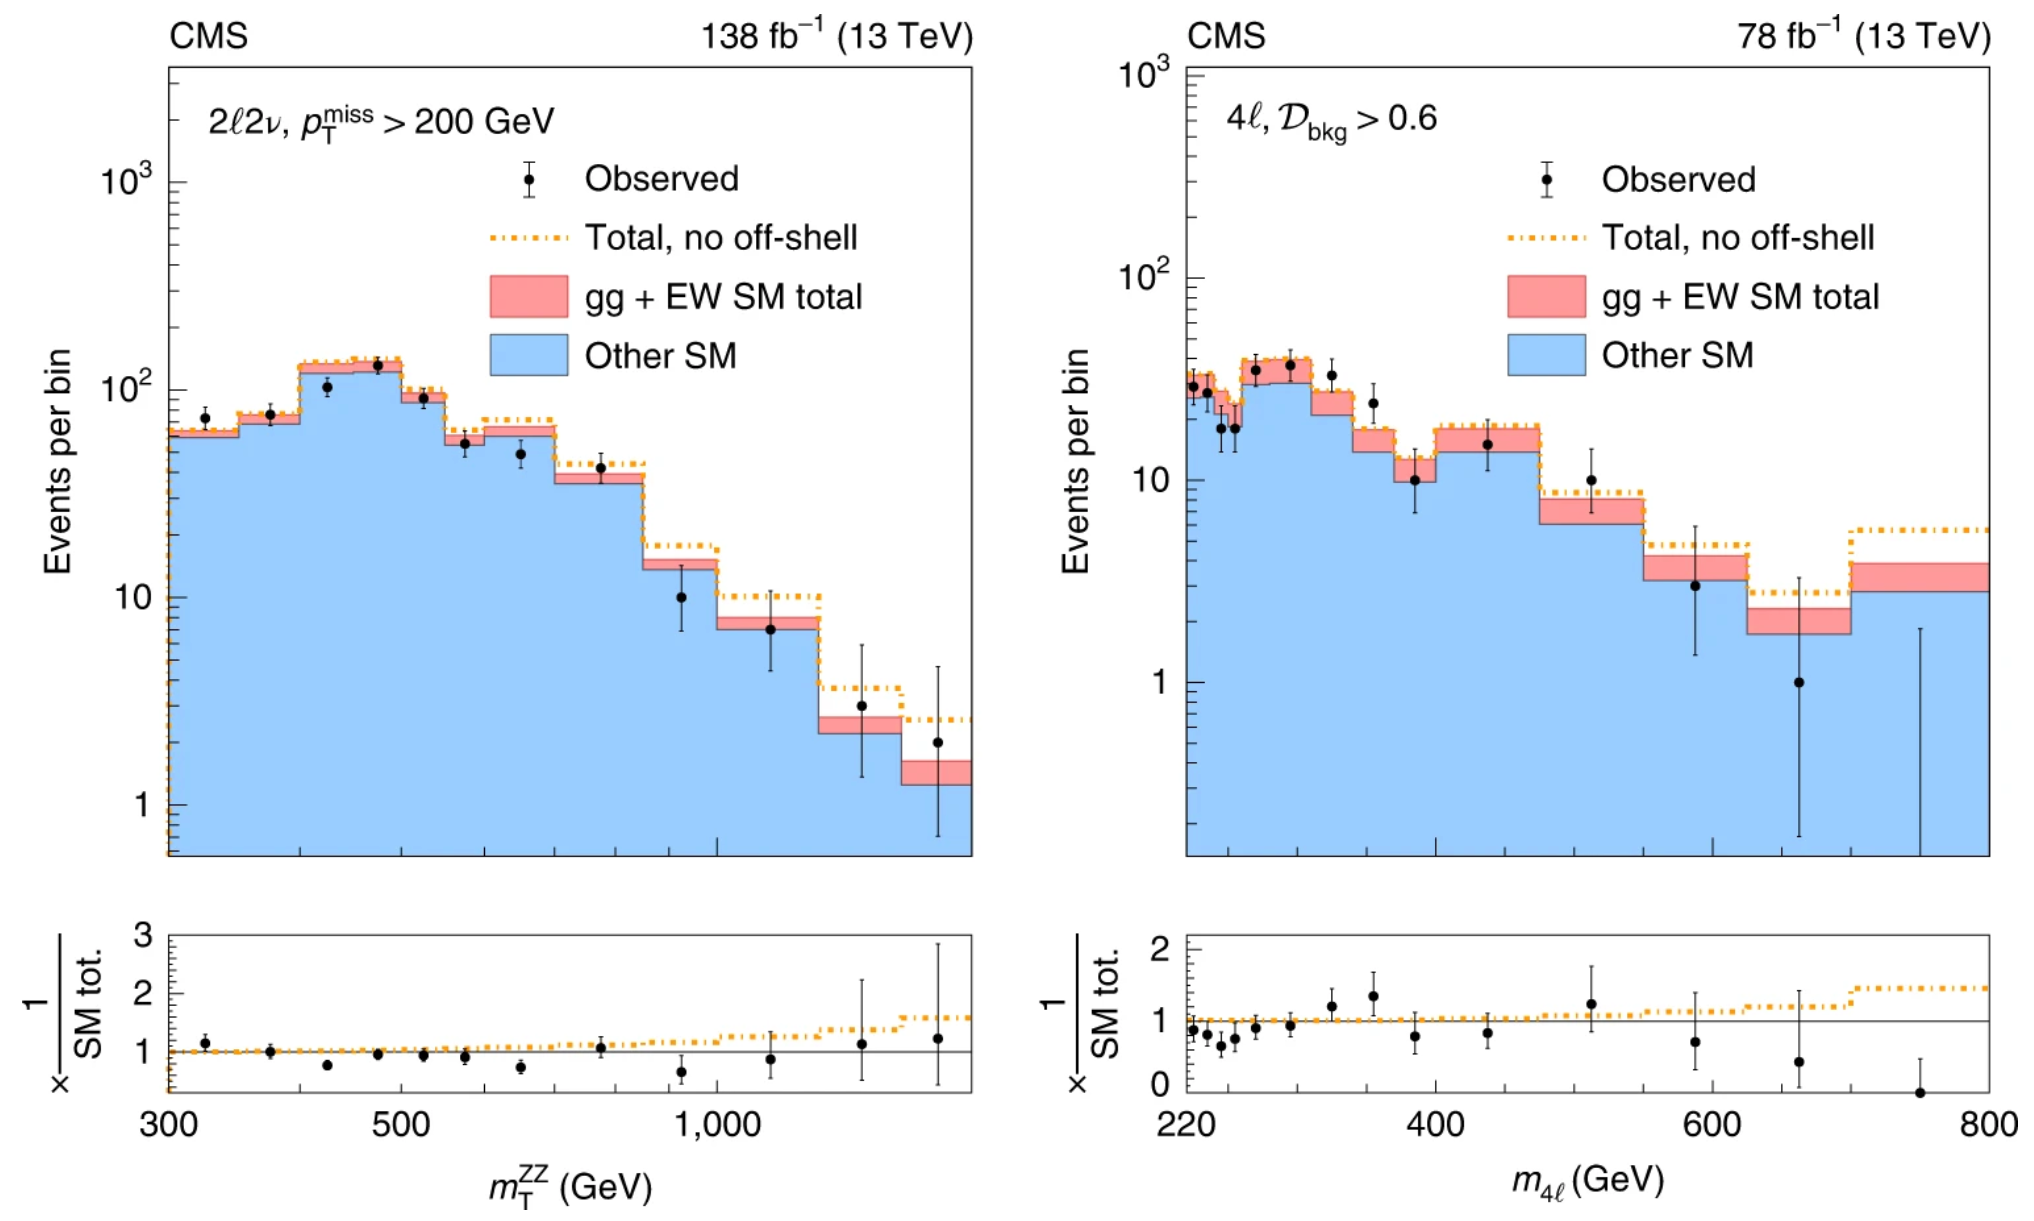
\includegraphics[width=0.9\linewidth]{figs/CMSOff.png}
  }\end{minipage}
}

\frame{
  \frametitle{Misure di precisione dell'Higgs: HL LHC}
  Autoaccoppiamento dell'Higgs.

  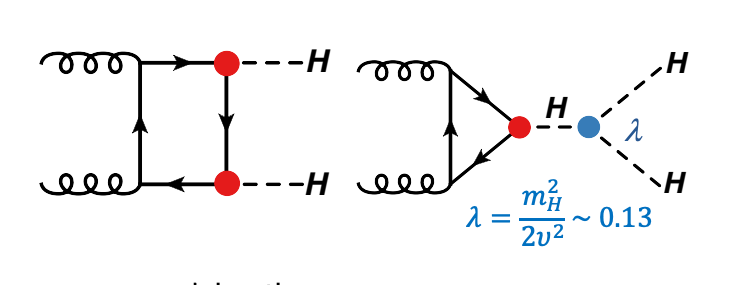
\includegraphics[width=0.3\linewidth]{figs/DIHiggs1.png}
  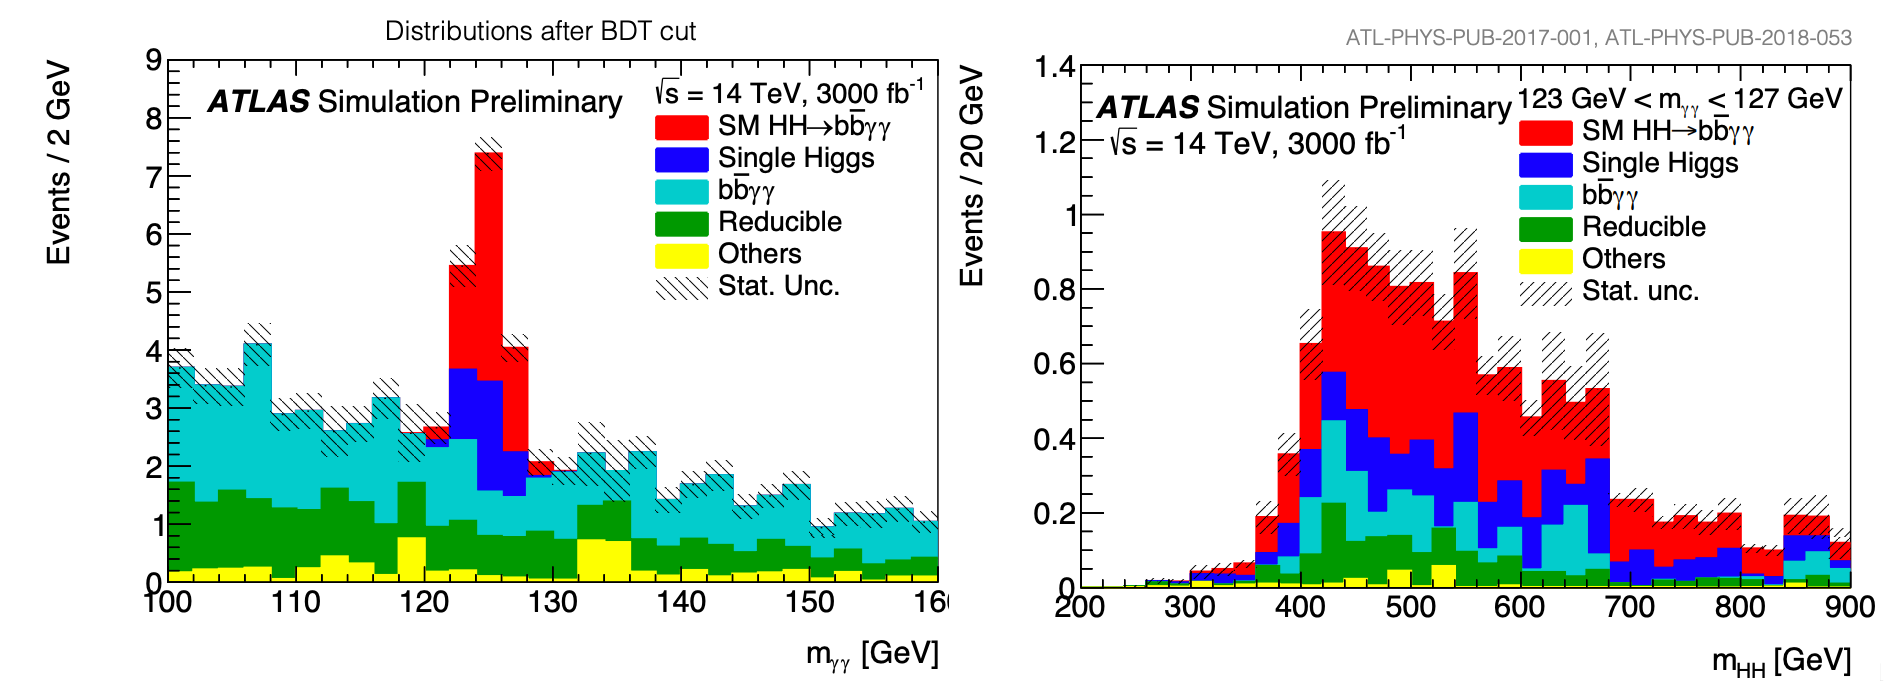
\includegraphics[width=0.8\linewidth]{figs/DIHiggs2.png}

  Molti altri canali a disposizione: $bbbb$, $bb\tau \tau$
  Necessarie analisi sofisticate: ampio spazio per innovazioni.
}

\frame{
  \frametitle{Altre misure/ricerche a HL-LHC (lista non esaustiva)}
  \footnotesize
  \begin{minipage}{0.65\linewidth}{
  \begin{itemize}
    \item Vector Boson Scattering (VBS)
    \item Forward-backward asymmetry in Drell-Yan dilepton events
    \item Massa del W e del top (proiezioni $m_W$ a 5~MeV)
    \item Eventi rari: tt+V, 4 top
    \item BSM resonance (incremento sensitivit\`a da 30\% a 70\%)
    \item Incremento sensibilit\`a ricerca SUSY
    \item Ricerca Dark matter (mono-X, X=Z,H,top)
    \item QCD and PDF determination
    \item Flavour Physics
  \end{itemize}
  }\end{minipage}\begin{minipage}{0.35\linewidth}{
    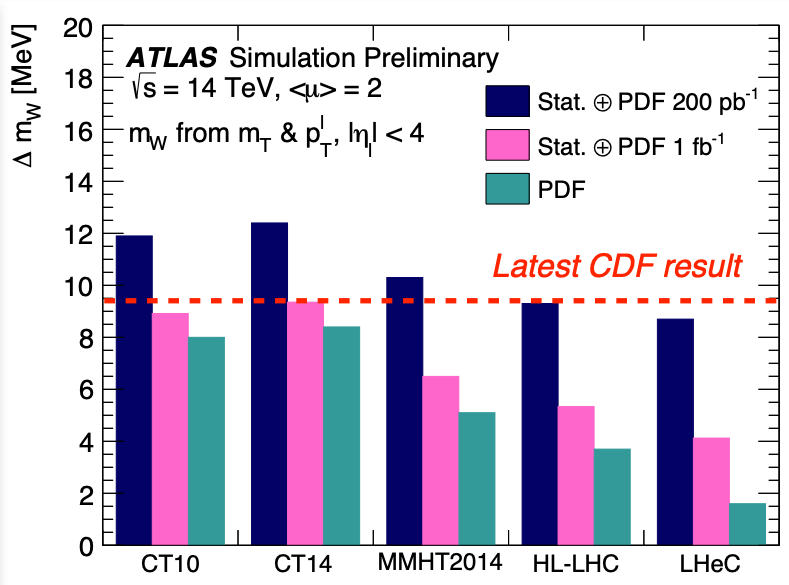
\includegraphics[width=0.6\linewidth]{figs/MW.png}
    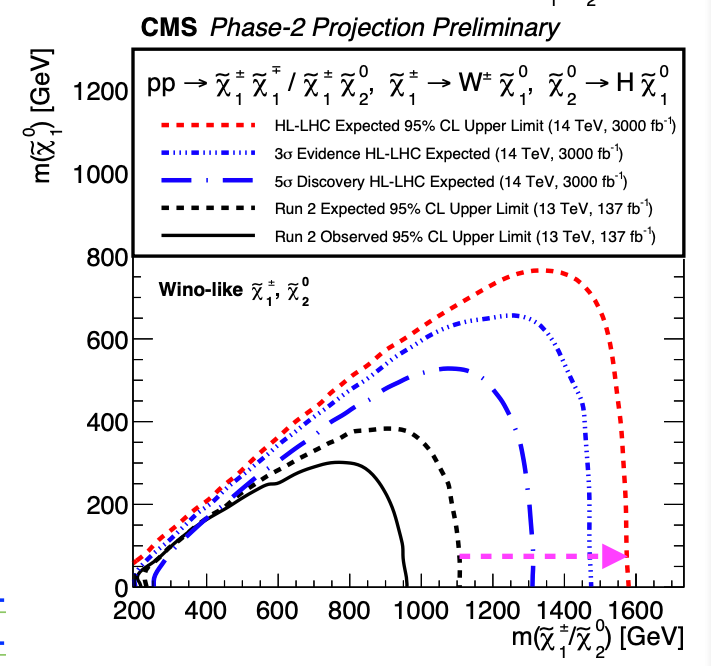
\includegraphics[width=0.6\linewidth]{figs/chi0.png}
  }\end{minipage}
}
